%=================================================================
% CSE 4345 — Big Data Analytics
% Week 6, Part 1: Apache Spark — RDDs, DataFrames,
%                 and In-Memory Computing
% Department of CSE, Premier University
%
% Part 1 covers: MapReduce disk bottleneck · Spark history & architecture
%               · RDD abstraction · Lineage fault tolerance
%               · Transformations vs actions · Lazy evaluation
%               · Narrow vs wide dependencies · Spark SQL / DataFrames
%               · Ecosystem (MLlib, Streaming) · Ivy League alignment · Assessment
% Part 2 covers: Zaharia et al. 2010 & 2012 papers · Databricks benchmark case study
%=================================================================

\documentclass[aspectratio=169,10pt]{beamer}

%---------- Packages ----------
\usepackage[utf8]{inputenc}
\usepackage[T1]{fontenc}
\usepackage{booktabs}
\usepackage{xcolor}
\usepackage{tikz}
\usetikzlibrary{shapes.geometric, positioning, arrows.meta,
                decorations.pathreplacing, calc, fit, backgrounds}
\usepackage{amsmath}
\usepackage{graphicx}
\usepackage{multicol}
\usepackage{enumerate}
\usepackage{array}
\usepackage{listings}

%---------- Theme ----------
\usetheme{Madrid}

%---------- Premier University Color Identity ----------
\definecolor{PUNavy}{RGB}{10,36,99}
\definecolor{PUGold}{RGB}{197,151,37}
\definecolor{PULightBlue}{RGB}{210,228,255}
\definecolor{PUTeal}{RGB}{0,100,100}
\definecolor{PUGray}{RGB}{90,90,90}
\definecolor{PURed}{RGB}{160,30,30}
\definecolor{PUGreen}{RGB}{30,120,60}
\definecolor{PUOrange}{RGB}{200,100,20}
\definecolor{PUPurple}{RGB}{80,0,120}

\setbeamercolor{palette primary}{bg=PUNavy, fg=white}
\setbeamercolor{palette secondary}{bg=PUNavy!85, fg=white}
\setbeamercolor{palette tertiary}{bg=PUNavy!70, fg=white}
\setbeamercolor{palette quaternary}{bg=PUNavy, fg=white}
\setbeamercolor{structure}{fg=PUNavy}
\setbeamercolor{title}{bg=PUNavy, fg=PUGold}
\setbeamercolor{subtitle}{fg=white}
\setbeamercolor{frametitle}{bg=PUNavy, fg=PUGold}
\setbeamercolor{alerted text}{fg=PUGold!85!black}
\setbeamercolor{block title}{bg=PUNavy, fg=white}
\setbeamercolor{block body}{bg=PULightBlue!45}
\setbeamercolor{block title alerted}{bg=PUGold!80!black, fg=white}
\setbeamercolor{block body alerted}{bg=PUGold!12}
\setbeamercolor{block title example}{bg=PUTeal, fg=white}
\setbeamercolor{block body example}{bg=PUTeal!10}
\setbeamercolor{section in toc}{fg=PUNavy}
\setbeamercolor{itemize item}{fg=PUGold!80!black}
\setbeamercolor{itemize subitem}{fg=PUNavy!70}

\setbeamertemplate{navigation symbols}{}
\setbeamertemplate{itemize item}{\scriptsize\raise1.5pt\hbox{\textbullet}}
\setbeamertemplate{itemize subitem}{\scriptsize\raise1pt\hbox{--}}

%---------- Code listing style ----------
\lstset{
  basicstyle=\ttfamily\scriptsize,
  backgroundcolor=\color{PUNavy!8},
  frame=single,
  rulecolor=\color{PUNavy!30},
  breaklines=true,
  language={},
  keywordstyle=\color{PUNavy}\bfseries,
  commentstyle=\color{PUGray}\itshape,
  stringstyle=\color{PUGreen!70!black},
}

%---------- Section separator ----------
\AtBeginSection[]{
  \begin{frame}[plain]
    \vfill\centering
    \begin{beamercolorbox}[sep=12pt,center,shadow=true,rounded=true]{block title}
      \usebeamerfont{title}\insertsectionhead\par
    \end{beamercolorbox}
    \vfill
  \end{frame}
}

%---------- Title metadata ----------
\title[CSE 4345 \textbar{} Week 6, Part 1]{CSE 4345: Big Data Analytics}
\subtitle{Week 6, Part 1 \textemdash\ Apache Spark:
          RDDs, DataFrames \& In-Memory Computing}
\author[Dept.\ of CSE]{Department of Computer Science \& Engineering\\[4pt]
       \small Premier University, Chittagong}
\institute{}
\date{Semester 2026}

%=================================================================
\begin{document}
%=================================================================

%----------------------------------------------------------------
\begin{frame}
  \titlepage
\end{frame}

%----------------------------------------------------------------
\begin{frame}{Course \& Lecture Information}
  \begin{columns}[T]
    \column{0.47\textwidth}
      \begin{block}{Lecture Identity}
        \begin{tabular}{ll}
          \textbf{Course:}      & CSE 4345 \\
          \textbf{Week / Part:} & 6 of 11 \textbar\ Part 1 of 2 \\
          \textbf{CLO:}         & CLO3 \\
          \textbf{PLO:}         & PLO(e), PLO(f) \\
        \end{tabular}
      \end{block}
      \vspace{6pt}
      \begin{alertblock}{CLO3}
        \textit{``Explain big data techniques, tools, and technologies used to store, manage, and analyse large datasets''}
      \end{alertblock}
      \vspace{6pt}
      \begin{block}{Course Progression}
        \small
        Week 4: MapReduce, Pig, Hive, HBase\\
        Week 5: YARN, file formats, compression\\
        \textbf{Week 6: Apache Spark — in-memory computing}\\
        Week 7: HiveQL, partitioning, Presto
      \end{block}
    \column{0.50\textwidth}
      \begin{exampleblock}{Part 1 Covers}
        \begin{itemize}
          \item Why MapReduce fails for iterative algorithms
          \item Spark history and the in-memory insight
          \item Spark architecture: Driver, Executors, Cluster Manager
          \item RDD: the core abstraction (immutable, partitioned, lineage)
          \item RDD lineage and fault-tolerant recomputation
          \item Transformations vs.\ actions; lazy evaluation
          \item Narrow vs.\ wide dependencies; stages and tasks
          \item PySpark programming examples
          \item Spark SQL and the DataFrame API
          \item Spark ecosystem (MLlib, Structured Streaming)
          \item Ivy League alignment
          \item Student assessment pool
        \end{itemize}
      \end{exampleblock}
  \end{columns}
\end{frame}

%----------------------------------------------------------------
\begin{frame}{Lecture Agenda}
  \tableofcontents
\end{frame}

%================================================================
\section{The MapReduce Bottleneck}
%================================================================

\begin{frame}{Why MapReduce Fails for Iterative Algorithms}
  \begin{columns}[T]
    \column{0.52\textwidth}
      \begin{block}{The Fundamental Problem}
        MapReduce writes \textbf{every intermediate result to HDFS} before the next step can begin.  For algorithms that must pass over the same data repeatedly (machine learning, graph algorithms), this incurs enormous disk I/O cost.
      \end{block}
      \vspace{4pt}
      \begin{exampleblock}{K-Means Clustering: 100 Iterations}
        \small Each iteration: read training data $\to$ compute new centroids $\to$ write to HDFS.
        \vspace{4pt}
        \begin{itemize}
          \item Dataset: 50 GB on HDFS
          \item \textbf{MapReduce}: 100 iterations $\times$ (50 GB read + 50 GB write) = \textbf{10 TB disk I/O}
          \item \textbf{Spark}: iteration 1 reads 50 GB from HDFS and caches in RAM.  Iterations 2--100 read from memory.  Total HDFS I/O: \textbf{50 GB} (initial read only)
          \item \textbf{Speedup: $\approx 200\times$ less disk I/O}
        \end{itemize}
      \end{exampleblock}

    \column{0.45\textwidth}
      \begin{center}
      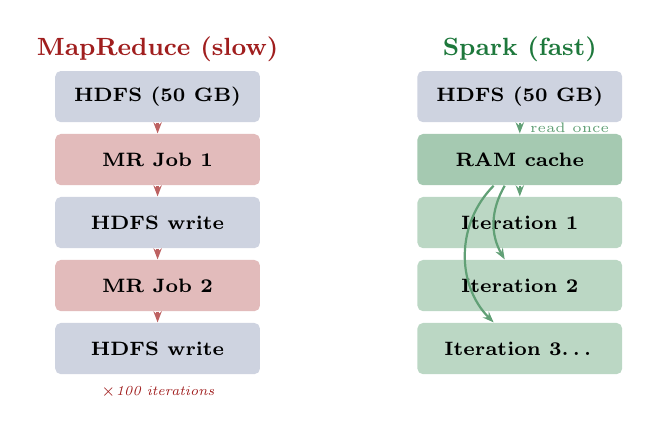
\begin{tikzpicture}[
          box/.style={rectangle, rounded corners=2pt, minimum width=2.6cm,
                      minimum height=0.65cm, font=\scriptsize\bfseries, align=center},
          arr/.style={-{Stealth[length=4pt]}, thick},
          io/.style={font=\tiny\itshape, PURed}
        ]
        % MapReduce iterative path
        \node[font=\small\bfseries, PURed] at (-0.2, 4.5) {MapReduce (slow)};
        \node[box, fill=PUNavy!20] (hdfs1) at (-0.2, 3.9) {HDFS (50 GB)};
        \node[box, fill=PURed!30]  (mr1)   at (-0.2, 3.1) {MR Job 1};
        \node[box, fill=PUNavy!20] (hdfs2) at (-0.2, 2.3) {HDFS write};
        \node[box, fill=PURed!30]  (mr2)   at (-0.2, 1.5) {MR Job 2};
        \node[box, fill=PUNavy!20] (hdfs3) at (-0.2, 0.7) {HDFS write};
        \node[io] at (-0.2, 0.15) {$\times$100 iterations};
        \draw[arr, PURed!70] (hdfs1)--(mr1);
        \draw[arr, PURed!70] (mr1)--(hdfs2);
        \draw[arr, PURed!70] (hdfs2)--(mr2);
        \draw[arr, PURed!70] (mr2)--(hdfs3);

        % Spark iterative path
        \node[font=\small\bfseries, PUGreen] at (4.4, 4.5) {Spark (fast)};
        \node[box, fill=PUNavy!20]  (shdfs) at (4.4, 3.9) {HDFS (50 GB)};
        \node[box, fill=PUGreen!40] (ram)   at (4.4, 3.1) {RAM cache};
        \node[box, fill=PUGreen!30] (sp1)   at (4.4, 2.3) {Iteration 1};
        \node[box, fill=PUGreen!30] (sp2)   at (4.4, 1.5) {Iteration 2};
        \node[box, fill=PUGreen!30] (sp3)   at (4.4, 0.7) {Iteration 3\ldots};
        \draw[arr, PUGreen!70] (shdfs)--(ram)
              node[midway,right,font=\tiny]{read once};
        \draw[arr, PUGreen!70] (ram)--(sp1);
        \draw[arr, PUGreen!70, bend right=30] (ram) to (sp2);
        \draw[arr, PUGreen!70, bend right=45] (ram) to (sp3);
      \end{tikzpicture}
      \end{center}
  \end{columns}
\end{frame}

%================================================================
\section{Apache Spark: Architecture \& RDDs}
%================================================================

\begin{frame}{Spark History and the In-Memory Insight}
  \begin{columns}[T]
    \column{0.52\textwidth}
      \begin{block}{Origin: UC Berkeley AMPLab (2009--2013)}
        \begin{itemize}
          \item \textbf{2009}: Matei Zaharia, PhD student at UC Berkeley, observes MapReduce is inefficient for iterative ML and interactive queries
          \item \textbf{2010}: First Spark paper (HotCloud 2010) — \textit{``Cluster Computing with Working Sets''}
          \item \textbf{2012}: RDD paper (NSDI 2012) formalises fault tolerance via \textbf{lineage} — Best Paper Award
          \item \textbf{2013}: Spark donated to Apache Software Foundation; Databricks founded
          \item \textbf{2014}: Spark sets world record in 100 TB sort benchmark (23 min vs.\ 72 min for Hadoop)
          \item \textbf{2016--present}: Default big data engine at Netflix, LinkedIn, Alibaba, Uber
        \end{itemize}
      \end{block}

    \column{0.45\textwidth}
      \begin{alertblock}{The Core Insight}
        \begin{quote}
          \itshape ``We introduce the concept of \textbf{resilient distributed datasets} (RDDs), a distributed memory abstraction that lets programmers perform in-memory computations on large clusters in a fault-tolerant manner.''
        \end{quote}
        \hfill --- Zaharia et al., NSDI 2012
      \end{alertblock}
      \vspace{6pt}
      \begin{exampleblock}{Why It Matters for Bangladesh}
        \small Bangladesh's largest ML use cases (fraud detection at bKash, disease prediction at DGHS, ride-demand forecasting at Pathao) all involve iterative algorithms over large datasets.  These are \textbf{exactly} the workloads where Spark outperforms MapReduce by orders of magnitude.
      \end{exampleblock}
  \end{columns}
\end{frame}

%----------------------------------------------------------------
\begin{frame}{Spark Architecture}
  \begin{columns}[T]
    \column{0.50\textwidth}
      \begin{block}{Three-Tier Architecture}
        \begin{enumerate}
          \item \textbf{Driver Program}: runs the user's \texttt{main()} function; creates \texttt{SparkContext}; builds the DAG of transformations; coordinates execution
          \item \textbf{Cluster Manager}: allocates resources across the cluster (YARN, Kubernetes, Mesos, or Spark Standalone)
          \item \textbf{Executors}: JVM processes launched on Worker Nodes; execute tasks; store cached RDD partitions in memory
        \end{enumerate}
      \end{block}
      \vspace{4pt}
      \begin{alertblock}{SparkContext vs.\ SparkSession}
        \small In Spark 1.x, \texttt{SparkContext} was the entry point.  In Spark 2.x+, \texttt{SparkSession} unifies SQL, DataFrames, and RDDs under one entry point.  \texttt{SparkContext} is still accessible as \texttt{spark.sparkContext}.
      \end{alertblock}

    \column{0.47\textwidth}
      \begin{center}
      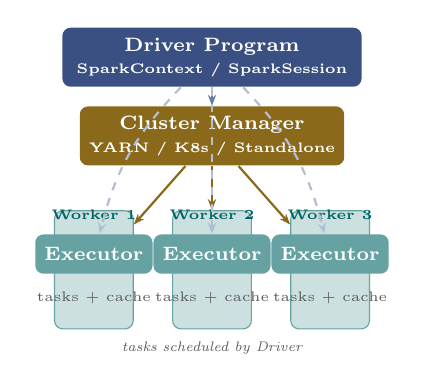
\begin{tikzpicture}[
          box/.style={rectangle, rounded corners=3pt,
                      minimum width=2.6cm, minimum height=0.75cm,
                      font=\scriptsize\bfseries, align=center},
          arr/.style={-{Stealth[length=4pt]}, thick}
        ]
        % Driver
        \node[box, fill=PUNavy!80, text=white, minimum width=3.8cm]
              (drv) at (2.0, 4.5) {Driver Program\\{\tiny SparkContext / SparkSession}};

        % Cluster Manager
        \node[box, fill=PUGold!70!black, text=white, minimum width=3.2cm]
              (cm) at (2.0, 3.5) {Cluster Manager\\{\tiny YARN / K8s / Standalone}};
        \draw[arr, PUNavy!60] (drv) -- (cm);

        % Workers
        \foreach \i/\x in {1/0.5, 2/2.0, 3/3.5} {
          \node[box, fill=PUTeal!20, draw=PUTeal!60,
                minimum height=1.5cm, minimum width=1.0cm]
                (wk\i) at (\x, 1.8) {};
          \node[font=\tiny\bfseries, PUTeal] at (\x, 2.5) {Worker \i};
          \node[box, fill=PUTeal!60, text=white,
                minimum width=0.8cm, minimum height=0.5cm]
                (ex\i) at (\x, 2.0) {Executor};
          \node[font=\tiny, PUGray] at (\x, 1.45) {tasks + cache};
          \draw[arr, PUGold!70!black] (cm) -- (wk\i);
        }

        % Task arrows from Driver to Executors
        \draw[arr, PUNavy!30, dashed, bend right=15] (drv) to (ex1);
        \draw[arr, PUNavy!30, dashed]                (drv) to (ex2);
        \draw[arr, PUNavy!30, dashed, bend left=15]  (drv) to (ex3);
        \node[font=\tiny\itshape, PUGray] at (2.0, 0.8)
              {tasks scheduled by Driver};
      \end{tikzpicture}
      \end{center}
  \end{columns}
\end{frame}

%----------------------------------------------------------------
\begin{frame}{Resilient Distributed Datasets (RDDs)}
  \begin{columns}[T]
    \column{0.52\textwidth}
      \begin{block}{Definition (Zaharia et al., 2012)}
        An RDD is a \textbf{read-only, partitioned collection of records} that can only be created by:
        \begin{enumerate}
          \item Transforming an existing RDD (e.g., \texttt{map}, \texttt{filter})
          \item Loading data from stable storage (e.g., HDFS, S3)
        \end{enumerate}
        \vspace{4pt}
        \textbf{Five key properties:}
        \begin{itemize}
          \item \textbf{Immutable}: never modified in place; transformations create new RDDs
          \item \textbf{Partitioned}: split across Executors for parallel processing
          \item \textbf{Lazy}: transformations only execute when an action is called
          \item \textbf{Lineage}: knows exactly how it was derived from its parent RDDs
          \item \textbf{Resilient}: lost partitions are recomputed from lineage, not replicated
        \end{itemize}
      \end{block}

    \column{0.45\textwidth}
      \begin{exampleblock}{What ``Resilient'' Actually Means}
        \small Traditional fault tolerance = \textbf{replicate data} (3 copies, like HDFS).\\
        RDD fault tolerance = \textbf{re-derive data} from its lineage (the computation graph).
        \vspace{6pt}

        If Partition 3 of an RDD is lost:
        \begin{enumerate}
          \item Spark reads the original HDFS input for that partition
          \item Re-applies the same sequence of transformations
          \item Result: the lost partition is regenerated
        \end{enumerate}
        \textbf{No data replication overhead.  The computation is the backup.}
      \end{exampleblock}
      \vspace{4pt}
      \begin{alertblock}{The Key Trade-off}
        \small Lineage-based recovery is efficient for \textbf{narrow} dependencies but expensive for \textbf{wide} dependencies (many ancestors to recompute).  Long lineage chains should be \textbf{checkpointed} to HDFS.
      \end{alertblock}
  \end{columns}
\end{frame}

%----------------------------------------------------------------
\begin{frame}{RDD Lineage: The Fault-Tolerance Mechanism}
  \begin{center}
  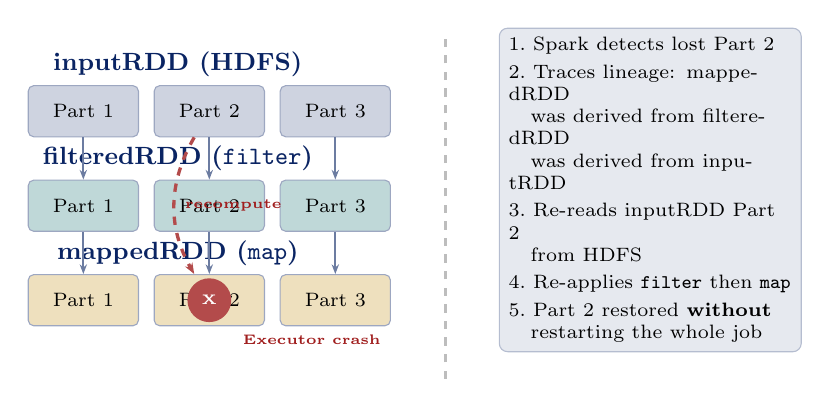
\begin{tikzpicture}[
      part/.style={rectangle, rounded corners=2pt, draw=PUNavy!40,
                   minimum width=1.4cm, minimum height=0.65cm,
                   font=\scriptsize, align=center},
      rddlbl/.style={font=\small\bfseries, PUNavy},
      arr/.style={-{Stealth[length=3.5pt]}, thick, PUNavy!60},
      fail/.style={circle, fill=PURed!80, text=white, minimum size=0.5cm,
                   font=\tiny\bfseries}
    ]
    % Row 1: input RDD
    \node[rddlbl] at (-0.2, 3.8) {inputRDD (HDFS)};
    \foreach \i/\x in {1/-1.4, 2/0.2, 3/1.8} {
      \node[part, fill=PUNavy!20] (in\i) at (\x, 3.2) {Part \i};
    }

    % Row 2: filteredRDD
    \node[rddlbl] at (-0.2, 2.6) {filteredRDD (\texttt{filter})};
    \foreach \i/\x in {1/-1.4, 2/0.2, 3/1.8} {
      \node[part, fill=PUTeal!25] (fl\i) at (\x, 2.0) {Part \i};
      \draw[arr] (in\i) -- (fl\i);
    }

    % Row 3: mappedRDD
    \node[rddlbl] at (-0.2, 1.4) {mappedRDD (\texttt{map})};
    \foreach \i/\x in {1/-1.4, 2/0.2, 3/1.8} {
      \node[part, fill=PUGold!30] (mp\i) at (\x, 0.8) {Part \i};
      \draw[arr] (fl\i) -- (mp\i);
    }

    % Failure on Part 2
    \node[fail] (x) at (0.2, 0.8) {X};
    \node[font=\tiny\bfseries, PURed] at (1.5, 0.3) {Executor crash};

    % Recovery arrow
    \draw[-{Stealth[length=4pt]}, PURed!80, very thick, dashed,
          bend right=30]
          (in2) to node[right, font=\tiny\bfseries, PURed]{recompute} (mp2);

    % Separator
    \draw[thick, PUGray!40, dashed] (3.2, -0.2) -- (3.2, 4.2);

    % Explanation
    \node[font=\small\bfseries, PUNavy] at (5.8, 3.8) {Recovery Path};
    \node[rectangle, fill=PUNavy!10, draw=PUNavy!30, rounded corners=3pt,
          minimum width=3.8cm, text width=3.6cm, font=\scriptsize, align=left]
          at (5.8, 2.2) {
      1.\ Spark detects lost Part 2\\[2pt]
      2.\ Traces lineage: mappedRDD\\
      \quad was derived from filteredRDD\\
      \quad was derived from inputRDD\\[2pt]
      3.\ Re-reads inputRDD Part 2\\
      \quad from HDFS\\[2pt]
      4.\ Re-applies \texttt{filter} then \texttt{map}\\[2pt]
      5.\ Part 2 restored \textbf{without}\\
      \quad restarting the whole job
    };
  \end{tikzpicture}
  \end{center}
\end{frame}

%================================================================
\section{Transformations, Actions, and Lazy Evaluation}
%================================================================

\begin{frame}{Transformations vs.\ Actions}
  \begin{columns}[T]
    \column{0.50\textwidth}
      \begin{block}{Transformations (Lazy)}
        Build the \textbf{computation DAG} but do not execute immediately.  Return a new RDD.
        \vspace{4pt}
        \renewcommand{\arraystretch}{1.2}
        \begin{tabular}{p{2.0cm}p{3.5cm}}
          \toprule
          \textbf{Transformation} & \textbf{What it does} \\
          \midrule
          \texttt{map(f)}     & Apply \texttt{f} to each element \\
          \texttt{filter(f)}  & Keep elements where \texttt{f} is True \\
          \texttt{flatMap(f)} & Map then flatten result \\
          \texttt{distinct()} & Remove duplicates \\
          \texttt{reduceByKey(f)} & Aggregate values per key \\
          \texttt{join(other)} & Inner join on key \\
          \texttt{groupByKey()} & Group values by key \\
          \texttt{cache()}    & Persist RDD in memory \\
          \bottomrule
        \end{tabular}
      \end{block}

    \column{0.47\textwidth}
      \begin{exampleblock}{Actions (Eager)}
        \textbf{Trigger execution} of the DAG.  Return a value to the Driver or write to storage.
        \vspace{4pt}
        \renewcommand{\arraystretch}{1.2}
        \begin{tabular}{p{2.3cm}p{2.5cm}}
          \toprule
          \textbf{Action} & \textbf{What it returns} \\
          \midrule
          \texttt{collect()}      & All elements (list) \\
          \texttt{count()}        & Number of elements \\
          \texttt{first()}        & First element \\
          \texttt{take(n)}        & First \texttt{n} elements \\
          \texttt{reduce(f)}      & Single aggregate value \\
          \texttt{saveAsTextFile} & Write to HDFS/disk \\
          \texttt{foreach(f)}     & Apply \texttt{f} side-effectfully \\
          \bottomrule
        \end{tabular}
        \vspace{4pt}
        \textbf{Rule:} \textit{No transformation executes until an action is called.}
      \end{exampleblock}
  \end{columns}
\end{frame}

%----------------------------------------------------------------
\begin{frame}{Lazy Evaluation: Why It Matters}
  \begin{columns}[T]
    \column{0.52\textwidth}
      \begin{block}{What Lazy Evaluation Means}
        When you call \texttt{rdd.filter(f).map(g)}, Spark does \textbf{nothing} yet.  It only records the computation graph (DAG).  When you call \texttt{.count()} or \texttt{.collect()}, Spark:
        \begin{enumerate}
          \item Analyses the full DAG
          \item Applies the \textbf{Catalyst optimizer} (for DataFrames) or Spark's DAG scheduler
          \item \textbf{Pipelines} compatible transformations: runs \texttt{filter} and \texttt{map} in a single pass over each partition — never writing intermediate results to disk
          \item Executes only the partitions needed
        \end{enumerate}
      \end{block}
      \vspace{4pt}
      \begin{alertblock}{Concrete Benefit}
        \small \texttt{rdd.filter(x > 1000).first()} — Spark stops after finding the \textbf{first matching element}.  Without lazy evaluation, it would filter the entire dataset first.
      \end{alertblock}

    \column{0.45\textwidth}
      \begin{center}
      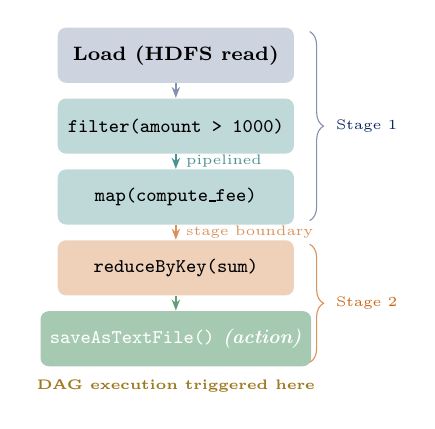
\begin{tikzpicture}[
          sbox/.style={rectangle, rounded corners=3pt, minimum width=3.0cm,
                       minimum height=0.7cm, font=\scriptsize\bfseries, align=center},
          arr/.style={-{Stealth[length=4pt]}, thick}
        ]
        \node[sbox, fill=PUNavy!20] (load) at (0,4.5)
              {Load (HDFS read)};
        \node[sbox, fill=PUTeal!25]  (flt)  at (0,3.6)
              {\texttt{filter(amount > 1000)}};
        \node[sbox, fill=PUTeal!25]  (mp)   at (0,2.7)
              {\texttt{map(compute\_fee)}};
        \node[sbox, fill=PUOrange!30] (rbk) at (0,1.8)
              {\texttt{reduceByKey(sum)}};
        \node[sbox, fill=PUGreen!40, text=white] (act) at (0,0.9)
              {\texttt{saveAsTextFile()} \textit{(action)}};
        \node[font=\tiny\bfseries, PUGold!80!black] at (0,0.3)
              {DAG execution triggered here};

        \draw[arr, PUNavy!50] (load)--(flt);
        \draw[arr, PUTeal!70] (flt)--(mp)
              node[midway,right,font=\tiny]{pipelined};
        \draw[arr, PUOrange!70] (mp)--(rbk)
              node[midway,right,font=\tiny]{stage boundary};
        \draw[arr, PUGreen!70] (rbk)--(act);

        % Stage brackets
        \draw[decorate, decoration={brace,amplitude=5pt}, PUNavy!50]
              (1.7,4.8) -- (1.7,2.4)
              node[midway,right=6pt,font=\tiny,text=PUNavy]{Stage 1};
        \draw[decorate, decoration={brace,amplitude=5pt}, PUOrange!70]
              (1.7,2.1) -- (1.7,0.6)
              node[midway,right=6pt,font=\tiny,text=PUOrange]{Stage 2};
      \end{tikzpicture}
      \end{center}
  \end{columns}
\end{frame}

%----------------------------------------------------------------
\begin{frame}{Narrow vs.\ Wide Dependencies: Stage Boundaries}
  \begin{columns}[T]
    \column{0.52\textwidth}
      \begin{block}{Narrow Dependencies (no shuffle)}
        Each output partition depends on \textbf{at most one} input partition.  Can be \textbf{pipelined} within a single stage.
        \vspace{4pt}
        \begin{itemize}
          \item \texttt{map}, \texttt{filter}, \texttt{flatMap}
          \item \texttt{union}, \texttt{mapPartitions}
          \item \texttt{coalesce} (reduce partitions, no shuffle)
        \end{itemize}
        \vspace{4pt}
        \textbf{Recovery}: if a partition is lost, recompute only that partition from its single parent partition.
      \end{block}
      \vspace{4pt}
      \begin{alertblock}{Wide Dependencies (requires shuffle)}
        Each output partition may depend on \textbf{multiple} input partitions.  Data must move across the network (shuffle).  Creates a \textbf{stage boundary}.
        \begin{itemize}
          \item \texttt{groupByKey}, \texttt{reduceByKey}, \texttt{aggregateByKey}
          \item \texttt{join} (without co-partitioning)
          \item \texttt{repartition}, \texttt{distinct}
        \end{itemize}
        \textbf{Recovery}: must recompute from all parent partitions (expensive).
      \end{alertblock}

    \column{0.45\textwidth}
      \begin{center}
      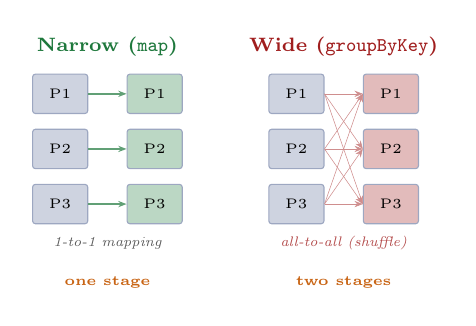
\begin{tikzpicture}[
          part/.style={rectangle, draw=PUNavy!40, fill=PUNavy!15,
                       minimum width=0.7cm, minimum height=0.5cm,
                       font=\tiny, rounded corners=1pt},
          arr/.style={-{Stealth[length=3pt]}, thick}
        ]
        % Narrow dependency (left)
        \node[font=\scriptsize\bfseries, PUGreen] at (-1.2, 3.9) {Narrow (\texttt{map})};
        \foreach \i/\y in {1/3.3, 2/2.6, 3/1.9} {
          \node[part, fill=PUNavy!20] (na\i) at (-1.8, \y) {P\i};
          \node[part, fill=PUGreen!30] (nb\i) at (-0.6, \y) {P\i};
          \draw[arr, PUGreen!70] (na\i)--(nb\i);
        }
        \node[font=\tiny\itshape, PUGray] at (-1.2,1.4)
              {1-to-1 mapping};

        % Wide dependency (right)
        \node[font=\scriptsize\bfseries, PURed] at (1.8, 3.9) {Wide (\texttt{groupByKey})};
        \foreach \i/\y in {1/3.3, 2/2.6, 3/1.9} {
          \node[part, fill=PUNavy!20] (wa\i) at (1.2, \y) {P\i};
          \node[part, fill=PURed!30]  (wb\i) at (2.4, \y) {P\i};
        }
        % All-to-all arrows
        \foreach \src in {1,2,3} {
          \foreach \dst in {1,2,3} {
            \draw[arr, PURed!50, very thin]
                  (wa\src.east) to (wb\dst.west);
          }
        }
        \node[font=\tiny\itshape, PURed!80] at (1.8,1.4)
              {all-to-all (shuffle)};

        % Stage markers
        \node[font=\tiny\bfseries, PUOrange] at (-1.2, 0.9) {one stage};
        \node[font=\tiny\bfseries, PUOrange] at (1.8,  0.9) {two stages};
      \end{tikzpicture}
      \end{center}
      \vspace{4pt}
      \begin{block}{Performance Tip}
        \small Prefer \texttt{reduceByKey} over \texttt{groupByKey}: \texttt{reduceByKey} applies a local combine before shuffling (like a Combiner in MapReduce), greatly reducing network traffic.
      \end{block}
  \end{columns}
\end{frame}

%================================================================
\section{PySpark Programming}
%================================================================

\begin{frame}[fragile]{PySpark: Word Count and Beyond}
  \begin{columns}[T]
    \column{0.50\textwidth}
      \begin{exampleblock}{Classic Word Count in PySpark}
        \begin{lstlisting}
from pyspark.sql import SparkSession

spark = SparkSession.builder \
    .appName("WordCount") \
    .getOrCreate()
sc = spark.sparkContext

# Load from HDFS
lines = sc.textFile(
    "hdfs:///data/corpus/*.txt")

# Transformations (lazy)
words   = lines.flatMap(
    lambda l: l.split())
pairs   = words.map(
    lambda w: (w, 1))
counts  = pairs.reduceByKey(
    lambda a, b: a + b)

# Action: write result
counts.saveAsTextFile(
    "hdfs:///output/wordcount/")
        \end{lstlisting}
      \end{exampleblock}

    \column{0.47\textwidth}
      \begin{exampleblock}{bKash Fraud Detection Pipeline}
        \begin{lstlisting}
# Load transaction records (Parquet)
txns = sc.textFile(
    "hdfs:///data/bkash/txns/")

# Parse CSV fields
def parse(line):
    f = line.split(",")
    return (f[0],       # txn_id
            f[1],       # sender
            float(f[2]))# amount

parsed = txns.map(parse)

# Flag suspicious: > 50000 BDT
# to new recipient in first txn
suspicious = parsed.filter(
    lambda r: r[2] > 50000.0)

# Count by sender
alerts = suspicious \
    .map(lambda r: (r[1], 1)) \
    .reduceByKey(lambda a,b: a+b) \
    .filter(lambda r: r[1] > 3)

print(alerts.count())  # action
        \end{lstlisting}
      \end{exampleblock}
  \end{columns}
\end{frame}

%================================================================
\section{Spark SQL and DataFrames}
%================================================================

\begin{frame}[fragile]{Spark SQL and the DataFrame API}
  \begin{columns}[T]
    \column{0.50\textwidth}
      \begin{block}{What is a DataFrame?}
        A \textbf{DataFrame} is a distributed collection of data organised into \textbf{named columns} with a schema — like a table in a relational database or a Pandas DataFrame, but distributed across a Spark cluster.
        \vspace{4pt}
        \begin{itemize}
          \item Built on top of RDDs internally
          \item Uses the \textbf{Catalyst optimizer}: rewrites query plans for maximum efficiency (predicate pushdown, join reordering, constant folding)
          \item Supports both \textbf{SQL} syntax and \textbf{Python/Scala} method chaining
          \item Reads Parquet, ORC, CSV, JSON, Hive tables, JDBC
        \end{itemize}
      \end{block}
      \vspace{4pt}
      \begin{alertblock}{DataFrame vs RDD}
        \small DataFrames are \textbf{10--100$\times$ faster} than RDDs for structured data because Catalyst can optimise the query before execution.  Use DataFrames/SQL unless you need low-level control.
      \end{alertblock}

    \column{0.47\textwidth}
      \begin{exampleblock}{DGHS Health Analytics (Spark SQL)}
        \begin{lstlisting}
# Load Parquet health records
df = spark.read.parquet(
    "hdfs:///data/dghs/records/")

# Register as SQL view
df.createOrReplaceTempView(
    "health_records")

# Query: district-wise disease count
result = spark.sql("""
  SELECT district,
         disease_code,
         COUNT(*) AS cases
  FROM   health_records
  WHERE  year = 2024
    AND  status = 'confirmed'
  GROUP BY district, disease_code
  ORDER BY cases DESC
  LIMIT 20
""")

# Write result as CSV
result.write \
    .mode("overwrite") \
    .csv("hdfs:///output/dghs/")
        \end{lstlisting}
      \end{exampleblock}
  \end{columns}
\end{frame}

%================================================================
\section{The Spark Ecosystem}
%================================================================

\begin{frame}{Spark Ecosystem: One Engine, Many Workloads}
  \begin{center}
  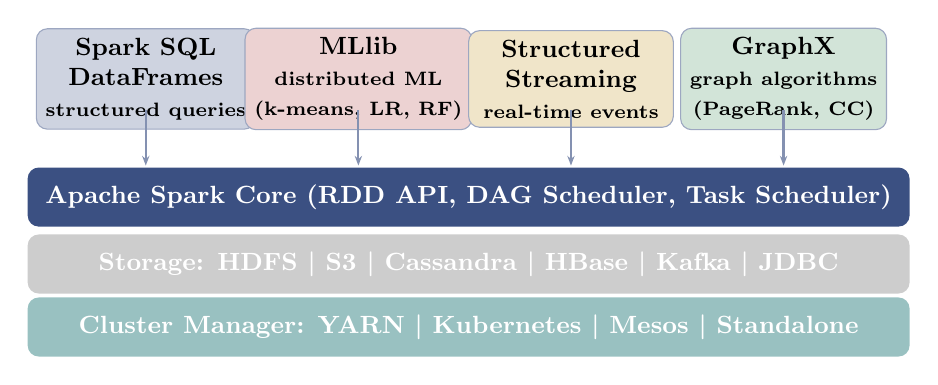
\begin{tikzpicture}[
      comp/.style={rectangle, rounded corners=4pt, draw=PUNavy!40,
                   minimum width=2.6cm, minimum height=1.1cm,
                   font=\small\bfseries, align=center},
      core/.style={rectangle, rounded corners=4pt, fill=PUNavy!80, text=white,
                   minimum width=11.2cm, minimum height=0.75cm,
                   font=\small\bfseries, align=center}
    ]
    % Core engine
    \node[core] (spark) at (0, 0.0)
          {Apache Spark Core (RDD API, DAG Scheduler, Task Scheduler)};

    % Four pillars
    \node[comp, fill=PUNavy!20]  at (-4.1, 1.5)
          {Spark SQL\\DataFrames\\{\scriptsize structured queries}};
    \node[comp, fill=PURed!20]   at (-1.4, 1.5)
          {MLlib\\{\scriptsize distributed ML}\\{\scriptsize (k-means, LR, RF)}};
    \node[comp, fill=PUGold!25]  at (1.3, 1.5)
          {Structured\\Streaming\\{\scriptsize real-time events}};
    \node[comp, fill=PUGreen!20] at (4.0, 1.5)
          {GraphX\\{\scriptsize graph algorithms}\\{\scriptsize (PageRank, CC)}};

    % Storage layer
    \node[core, fill=PUGray!30, minimum width=11.2cm] (storage) at (0, -0.85)
          {Storage: HDFS \textbar\ S3 \textbar\ Cassandra \textbar\ HBase \textbar\ Kafka \textbar\ JDBC};

    % Cluster managers
    \node[core, fill=PUTeal!40, minimum width=11.2cm] at (0, -1.65)
          {Cluster Manager: YARN \textbar\ Kubernetes \textbar\ Mesos \textbar\ Standalone};

    % Arrows
    \foreach \x in {-4.1,-1.4,1.3,4.0} {
      \draw[-{Stealth[length=3.5pt]}, PUNavy!50, thick] (\x, 1.1) -- (\x, 0.4);
    }
  \end{tikzpicture}
  \end{center}
  \vspace{4pt}
  \begin{columns}[T]
    \column{0.48\textwidth}
      \begin{block}{MLlib: Distributed Machine Learning}
        \small Supports classification, regression, clustering, dimensionality reduction, and collaborative filtering.  All algorithms are designed to run in-memory across the cluster, leveraging Spark's RDD caching for iterative training.
      \end{block}
    \column{0.48\textwidth}
      \begin{alertblock}{Structured Streaming}
        \small Treats a stream as a continuously-appended table; uses the same DataFrame/SQL API as batch.  Supports event-time windowing, watermarks for late data, and exactly-once processing with Kafka.
      \end{alertblock}
  \end{columns}
\end{frame}

%================================================================
\section{MapReduce vs.\ Spark: Head-to-Head}
%================================================================

\begin{frame}{MapReduce vs.\ Spark: Complete Comparison}
  \centering
  \renewcommand{\arraystretch}{1.45}
  \begin{tabular}{p{2.8cm}p{3.2cm}p{3.8cm}}
    \toprule
    \textbf{Dimension} & \textbf{MapReduce} & \textbf{Spark} \\
    \midrule
    Intermediate storage  & Disk (HDFS) after every step & Memory (spill to disk if needed) \\
    Programming model     & Map + Reduce only & map, filter, join, groupBy, SQL, ML, stream \\
    Languages             & Java (primary)    & Python, Scala, Java, R \\
    Iterative algorithms  & Slow (disk per iteration) & Fast (cache RDD; 10--100$\times$) \\
    Fault tolerance       & Re-execute task from HDFS & Recompute from lineage \\
    Stream processing     & Not supported natively & Structured Streaming (near real-time) \\
    Interactive queries   & Not feasible ($>$30 s)    & Spark Shell / Zeppelin (sub-second) \\
    Ecosystem integration & Pig, Hive, HBase  & Spark SQL, MLlib, GraphX, Delta Lake \\
    Learning curve        & Low (2 functions) & Moderate (rich API) \\
    \midrule
    \textbf{Use MapReduce when} & \multicolumn{2}{p{7.0cm}}{\small Single-pass batch jobs on very large clusters where Spark's memory overhead ($\sim$8 GB/Executor min) is prohibitive; or when existing MapReduce code is stable and fast enough} \\
    \textbf{Use Spark when} & \multicolumn{2}{p{7.0cm}}{\small ML training, graph processing, interactive analytics, streaming, or any workload with $>$2 iterations over the same data} \\
    \bottomrule
  \end{tabular}
\end{frame}

%================================================================
\section{Ivy League Alignment}
%================================================================

\begin{frame}{Spark in Top University Curricula}
  \begin{columns}[T]
    \column{0.55\textwidth}
      \begin{block}{Stanford CS246 (Leskovec) — Mining of Massive Datasets}
        \small The entire modern portion of CS246 is taught in \textbf{PySpark}:
        \begin{itemize}
          \item \textbf{RDD lineage} is covered as a formal directed acyclic graph (DAG) with typed edges (narrow vs.\ wide)
          \item \textbf{PageRank on Spark}: students implement the iterative algorithm and observe the 100$\times$ speedup vs.\ MapReduce because the graph adjacency matrix is cached
          \item \textbf{Homework assignments}: all submitted as PySpark notebooks run on a shared Spark cluster; students must justify every \texttt{cache()} call with a cost estimate
        \end{itemize}
        \textbf{Stanford exam question:} \textit{``Given the following Spark DAG, identify all stage boundaries and estimate the total shuffle volume for a 1 TB input dataset with 1{,}000 partitions.''}
      \end{block}

    \column{0.42\textwidth}
      \begin{exampleblock}{MIT 6.830 — Database Systems}
        \small MIT frames Spark as a \textbf{query engine with deferred execution}:
        \begin{itemize}
          \item Catalyst optimizer = a relational algebra rewriter
          \item DataFrame.explain() shows the physical plan — same concept as \texttt{EXPLAIN} in SQL databases
          \item Spark SQL closes the gap between MapReduce-style systems and MPP databases
        \end{itemize}
      \end{exampleblock}
      \vspace{4pt}
      \begin{alertblock}{CMU 15-721 — Advanced DB Systems (Pavlo)}
        \small CMU benchmarks Spark SQL against vectorised column-store engines (DuckDB, Velox).  Spark's JVM overhead and row-at-a-time RDD model are replaced by \textbf{Tungsten} (code generation) and \textbf{Photon} (native C++ execution in Databricks).  CMU teaches these as successive generations of the same system.
      \end{alertblock}
  \end{columns}
\end{frame}

%================================================================
\section{Student Assessment Pool}
%================================================================

\begin{frame}{Assessment\textemdash MCQ Set A \hfill\small\textit{CLO3}}
  \begin{exampleblock}{Instructions}
    Select the single best answer.  Correct answers \textbf{bolded} for instructor reference.
  \end{exampleblock}
  \vspace{8pt}
  \begin{itemize}
    \item[\textbf{Q1.}] What makes Spark significantly \textbf{faster than MapReduce} for iterative algorithms?
    \begin{enumerate}[(a)]
      \item Spark uses more CPU cores per node
      \item Spark writes intermediate results to faster SSDs
      \item \textbf{Spark caches intermediate data as RDDs in memory}
      \item Spark skips the shuffle phase entirely
    \end{enumerate}
  \end{itemize}
  \vspace{8pt}
  \begin{itemize}
    \item[\textbf{Q2.}] How does Spark achieve \textbf{fault tolerance} in RDDs \emph{without} full data replication?
    \begin{enumerate}[(a)]
      \item Checkpointing to HDFS every 60 seconds
      \item \textbf{Tracking lineage and recomputing lost partitions from parent RDDs}
      \item Copying each RDD partition twice across two Executors
      \item Using a write-ahead log on the Driver node
    \end{enumerate}
  \end{itemize}
  \vspace{8pt}
  \begin{alertblock}{Instructor Notes}
    \textbf{Q1:} Option (a) is a common distractor — Spark uses the same hardware as MapReduce.  The key is \textbf{memory, not cores}.  \textbf{Q2:} Option (c) describes replication (HDFS-style); option (a) describes checkpointing (used for long lineages, not the primary mechanism).  Lineage + recomputation (b) is the defining feature of RDDs.
  \end{alertblock}
\end{frame}

%----------------------------------------------------------------
\begin{frame}{Assessment\textemdash MCQ Set B \hfill\small\textit{CLO3}}
  \vspace{6pt}
  \begin{itemize}
    \item[\textbf{Q3.}] Which of the following is \textbf{NOT} a component of the Spark ecosystem?
    \begin{enumerate}[(a)]
      \item MLlib \quad (b) GraphX \quad (c) Structured Streaming \quad (d) \textbf{HBase}
    \end{enumerate}
  \end{itemize}
  \vspace{8pt}
  \begin{itemize}
    \item[\textbf{Q4.}] In Spark, a ``transformation'' such as \texttt{map()} or \texttt{filter()} is:
    \begin{enumerate}[(a)]
      \item Immediately executed when called and materialised to memory
      \item \textbf{Lazily evaluated --- only executed when a subsequent action is called}
      \item Automatically persisted to HDFS after execution
      \item Only available in the Scala API, not in PySpark
    \end{enumerate}
  \end{itemize}
  \vspace{8pt}
  \begin{alertblock}{Instructor Notes}
    \textbf{Q3:} HBase (option d) is a separate NoSQL database (covered in Week 4) that runs on HDFS.  It can be used as a \emph{data source} for Spark but is not part of the Spark ecosystem itself.  \textbf{Q4:} This is the fundamental ``lazy evaluation'' concept.  Students who answer (a) have a critical misconception that leads to inefficient Spark programs.  Show \texttt{rdd.filter().count()} vs.\ just \texttt{rdd.filter()} to demonstrate.
  \end{alertblock}
\end{frame}

%----------------------------------------------------------------
\begin{frame}{Assessment\textemdash True / False \hfill\small\textit{CLO3}}
  \begin{block}{Instructions}
    State True or False and provide a \textbf{one-sentence justification} for full marks.
  \end{block}
  \vspace{6pt}
  \centering
  \renewcommand{\arraystretch}{1.6}
  \begin{tabular}{p{9.2cm}c}
    \toprule
    \textbf{Statement} & \textbf{Answer} \\
    \midrule
    1.\ Spark can only run on top of Hadoop YARN and has no other deployment option. &
    \alert{\textbf{False}} \\
    2.\ RDDs are mutable — individual elements can be modified in place after creation. &
    \alert{\textbf{False}} \\
    3.\ Spark's DataFrame API provides schema-aware, named-column operations similar to SQL tables. &
    \textbf{True} \\
    4.\ MapReduce is generally better than Spark for machine learning workloads that require many iterations over the same dataset. &
    \alert{\textbf{False}} \\
    \bottomrule
  \end{tabular}
  \vspace{6pt}
  \begin{exampleblock}{Model Justifications}
    \small \textbf{1:} Spark supports YARN, Kubernetes, Apache Mesos, and Spark Standalone cluster managers.  \textbf{2:} RDDs are \textbf{immutable}; applying a transformation creates a \emph{new} RDD — the original is never modified.  \textbf{4:} For iterative ML, Spark is 10--100$\times$ faster because it caches the training data in memory; MapReduce re-reads from HDFS on every iteration.
  \end{exampleblock}
\end{frame}

%----------------------------------------------------------------
\begin{frame}{Assessment\textemdash Descriptive Questions \hfill\small\textit{CLO3}}
  \begin{block}{Instructions}
    Answer each question in \textbf{100--150 words}.  Include a diagram where indicated.
  \end{block}
  \vspace{8pt}
  \begin{itemize}
    \item[\textbf{D1.}] Explain the concept of a \textbf{Resilient Distributed Dataset (RDD)}.  What does \textit{``resilient''} mean in this context?  How does Spark recover a lost RDD partition without replication?
  \end{itemize}
  \vspace{8pt}
  \begin{itemize}
    \item[\textbf{D2.}] Differentiate between \textbf{Spark transformations} and \textbf{actions}.  Give two concrete examples of each.  Why does Spark not execute transformations immediately?
  \end{itemize}
  \vspace{8pt}
  \begin{itemize}
    \item[\textbf{D3.}] Describe Spark's \textbf{lazy evaluation model}.  What is the advantage of deferring computation until an action is called?  Use the example \texttt{rdd.filter(x > 1000).first()} to illustrate.
  \end{itemize}
\end{frame}

%----------------------------------------------------------------
\begin{frame}{Assessment\textemdash Analytical Questions \hfill\small\textit{CLO3}}
  \begin{block}{Instructions}
    Answer in \textbf{200--300 words} with step-by-step reasoning and quantified estimates.
  \end{block}
  \vspace{6pt}
  \begin{itemize}
    \item[\textbf{A1.}] \textbf{Iterative I/O Cost Analysis:}\\
    You need to train a K-Means clustering model over \textbf{50 GB} of bKash transaction data with \textbf{100 iterations}.  Assume HDFS read speed = 500 MB/s and RAM cache read speed = 5{,}000 MB/s.
    \begin{itemize}
      \item Calculate the total HDFS I/O for MapReduce (all 100 iterations)
      \item Calculate the total I/O for Spark (50 GB fits in cluster RAM)
      \item Estimate the wall-clock time for each approach
      \item Under what conditions would Spark NOT outperform MapReduce?
    \end{itemize}
  \end{itemize}
  \vspace{6pt}
  \begin{itemize}
    \item[\textbf{A2.}] \textbf{RDD Failure Recovery Trace:}\\
    A Spark job computes \texttt{input $\to$ filteredRDD $\to$ mappedRDD $\to$ reducedRDD} over 10 partitions.  Mid-execution, the Executor holding partitions 3 and 7 of \texttt{reducedRDD} crashes.  Trace the complete recovery sequence: what does the Driver detect, which partitions of which RDDs need to be recomputed, and what is the worst-case recovery cost if \texttt{reducedRDD} involves a \textbf{wide} dependency (\texttt{groupByKey})?
  \end{itemize}
\end{frame}

%================================================================
\section*{Textbook References}
%================================================================

\begin{frame}{Textbook \& Reading References}
  \begin{block}{Primary Textbooks for Week 6}
    \begin{itemize}
      \item \textbf{[TW]}\ Tom White. \textit{Hadoop: The Definitive Guide}, O'Reilly, 4th ed., 2015.
            \hfill \textbf{Ch.\ 2, 19}
            \begin{itemize}
              \small\item Ch.\,2: MapReduce (baseline for comparison) $\cdot$ Ch.\,19: Spark (appendix)
            \end{itemize}
      \item \textbf{[SA]}\ Acharya \& Chellappan. \textit{Big Data and Analytics}, Wiley, 2015.
            \hfill \textbf{Ch.\ 7}
            \begin{itemize}
              \small\item Ch.\,7: Introduction to Apache Spark
            \end{itemize}
      \item \textbf{[LRU]}\ Leskovec, Rajaraman \& Ullman. \textit{Mining of Massive Datasets}, 3rd ed.
            \hfill \textbf{Ch.\ 2.4}
            \begin{itemize}
              \small\item Ch.\,2.4: Spark's model; extensions beyond MapReduce
            \end{itemize}
    \end{itemize}
  \end{block}
  \vspace{6pt}
  \begin{exampleblock}{Supplementary (Covered in Week 6, Part 2 --- Seminal Papers)}
    \begin{itemize}
      \small
      \item Zaharia, M.\ et al.\ (2010). \textbf{Spark: Cluster Computing with Working Sets.}
            \textit{USENIX HotCloud 2010}.
      \item Zaharia, M.\ et al.\ (2012). \textbf{Resilient Distributed Datasets: A Fault-Tolerant Abstraction for In-Memory Cluster Computing.}
            \textit{USENIX NSDI 2012.}\ \textbf{Best Paper Award.}\ \textbf{[PRIMARY SEMINAL PAPER]}
      \item Karau, H.\ et al.\ \textit{Learning Spark}, O'Reilly, 2015 (1st ed.\ freely available as PDF).
    \end{itemize}
  \end{exampleblock}
\end{frame}

%----------------------------------------------------------------
\begin{frame}[c]
  \begin{center}
    {\Large\bfseries Questions \& Discussion}\\[10pt]
    {\large Week 6, Part 1 $\;\mid\;$ CSE 4345 Big Data Analytics}\\[8pt]
    \textcolor{PUGray}{\rule{7cm}{0.5pt}}\\[10pt]
    \begin{quote}
      \itshape ``We introduced RDDs to provide a programming model that allows users to explicitly control how data is cached in memory across operations --- a capability that simply did not exist in MapReduce.''
    \end{quote}
    \hfill\textemdash\,Matei Zaharia, NSDI 2012
    \vspace{12pt}
    \begin{block}{\centering Next Lecture: Week 6, Part 2}
      \centering
      Seminal Paper 1: Zaharia et al.\ (2010) --- \textit{``Spark: Cluster Computing with Working Sets''}\\[4pt]
      Seminal Paper 2: Zaharia et al.\ (2012) --- \textit{``Resilient Distributed Datasets''}\\[4pt]
      \small Case Study: Databricks logistic regression benchmark (2014) ---
      100$\times$ vs.\ Hadoop MapReduce on the same cluster
    \end{block}
    \vspace{6pt}
    \textbf{Reading before Part 2:}\ \textbf{[SA]} Ch.\,7 $\cdot$ Zaharia et al.\ (2012) RDD paper (see references)
  \end{center}
\end{frame}

%=================================================================
\end{document}
%=================================================================
